\documentclass{standalone}
\usepackage{tikz}
\usetikzlibrary{patterns, positioning}


\begin{document}
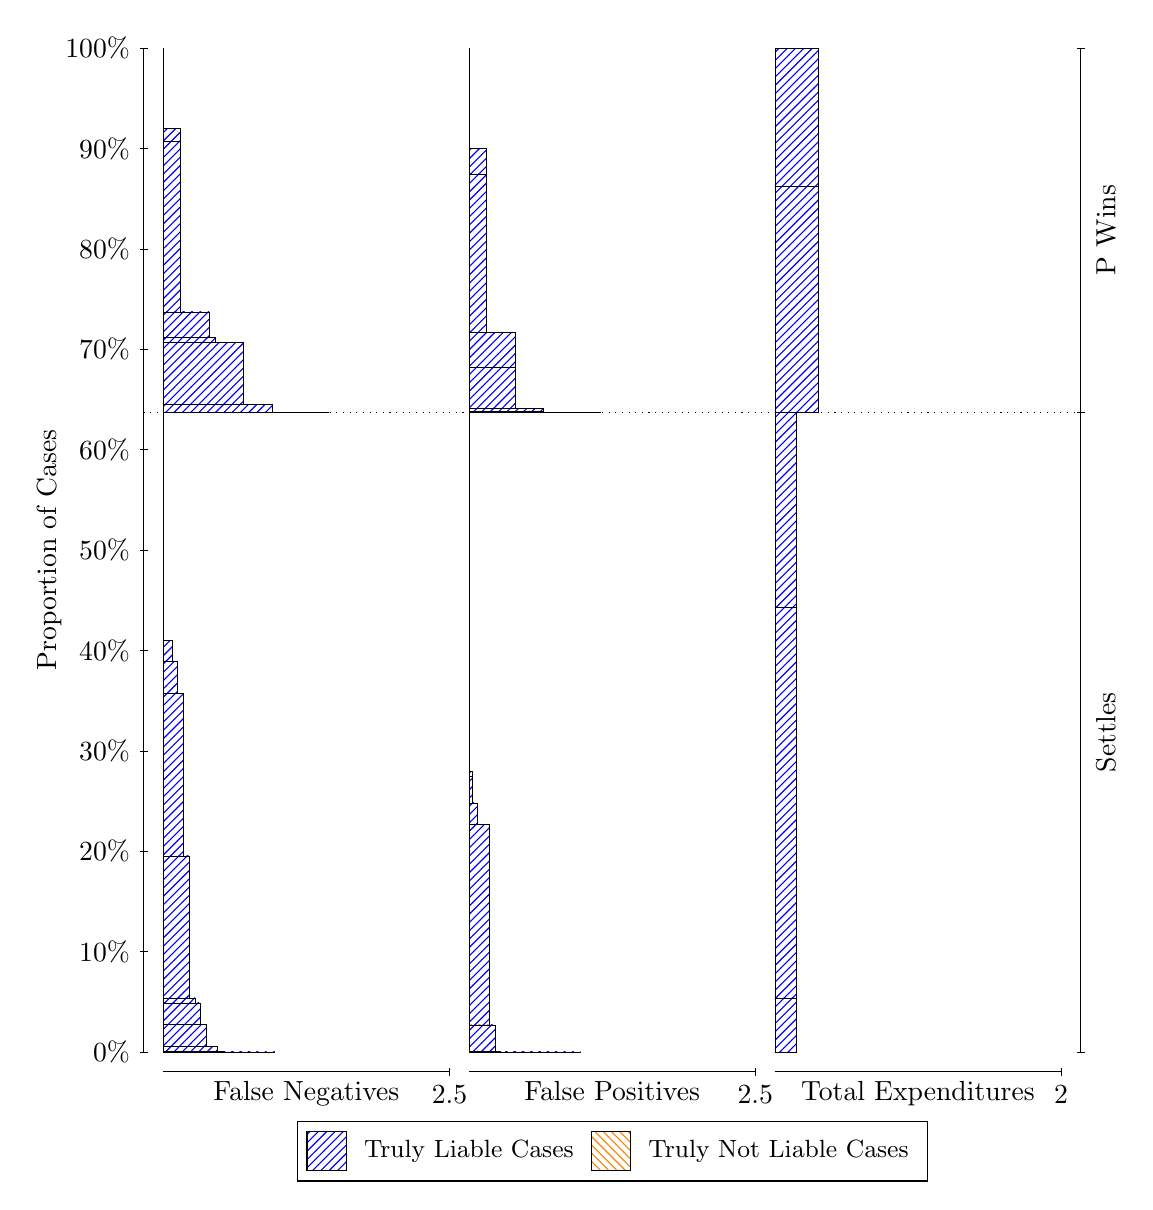
\begin{tikzpicture}
\draw[black, very thin] (1.5,1.75) -- (1.5,14.5);
\node[rotate=90, text=black, anchor=center] at (0.3, 8.125) {Proportion of Cases};
\draw[black, very thin] (1.45,1.75) -- (1.55,1.75);
\node[text=black, anchor=east] at (1.45, 1.75) {0\%};
\draw[black, very thin] (1.45,3.025) -- (1.55,3.025);
\node[text=black, anchor=east] at (1.45, 3.025) {10\%};
\draw[black, very thin] (1.45,4.3) -- (1.55,4.3);
\node[text=black, anchor=east] at (1.45, 4.3) {20\%};
\draw[black, very thin] (1.45,5.575) -- (1.55,5.575);
\node[text=black, anchor=east] at (1.45, 5.575) {30\%};
\draw[black, very thin] (1.45,6.85) -- (1.55,6.85);
\node[text=black, anchor=east] at (1.45, 6.85) {40\%};
\draw[black, very thin] (1.45,8.125) -- (1.55,8.125);
\node[text=black, anchor=east] at (1.45, 8.125) {50\%};
\draw[black, very thin] (1.45,9.4) -- (1.55,9.4);
\node[text=black, anchor=east] at (1.45, 9.4) {60\%};
\draw[black, very thin] (1.45,10.675) -- (1.55,10.675);
\node[text=black, anchor=east] at (1.45, 10.675) {70\%};
\draw[black, very thin] (1.45,11.95) -- (1.55,11.95);
\node[text=black, anchor=east] at (1.45, 11.95) {80\%};
\draw[black, very thin] (1.45,13.225) -- (1.55,13.225);
\node[text=black, anchor=east] at (1.45, 13.225) {90\%};
\draw[black, very thin] (1.45,14.5) -- (1.55,14.5);
\node[text=black, anchor=east] at (1.45, 14.5) {100\%};

\draw[black, very thin] (13.4,1.75) -- (13.4,14.5);
\draw[black, very thin] (13.35,1.75) -- (13.45,1.75);
\node[anchor=west] at (13.35, 1.75) {};
\draw[black, very thin] (13.35,9.8717) -- (13.45,9.8717);
\node[anchor=west] at (13.35, 9.8717) {};
\draw[black, very thin] (13.35,14.5) -- (13.45,14.5);
\node[anchor=west] at (13.35, 14.5) {};

\draw[black, very thin, pattern color=blue, pattern=north east lines] (1.75,1.75) rectangle (3.167,1.75);
\draw[black, very thin, pattern color=blue, pattern=north east lines] (1.75,1.75) rectangle (3.0217,1.75);
\draw[black, very thin, pattern color=blue, pattern=north east lines] (1.75,1.75) rectangle (2.8763,1.75);
\draw[black, very thin, pattern color=blue, pattern=north east lines] (1.75,1.75) rectangle (2.8037,1.75);
\draw[black, very thin, pattern color=blue, pattern=north east lines] (1.75,1.75) rectangle (2.6583,1.7505);
\draw[black, very thin, pattern color=blue, pattern=north east lines] (1.75,1.7505) rectangle (2.5857,1.7513);
\draw[black, very thin, pattern color=blue, pattern=north east lines] (1.75,1.7513) rectangle (2.513,1.7537);
\draw[black, very thin, pattern color=blue, pattern=north east lines] (1.75,1.7537) rectangle (2.4403,1.8179);
\draw[black, very thin, pattern color=blue, pattern=north east lines] (1.75,1.8179) rectangle (2.295,2.0974);
\draw[black, very thin, pattern color=blue, pattern=north east lines] (1.75,2.0974) rectangle (2.2223,2.3725);
\draw[black, very thin, pattern color=blue, pattern=north east lines] (1.75,2.3725) rectangle (2.1497,2.4362);
\draw[black, very thin, pattern color=blue, pattern=north east lines] (1.75,2.4362) rectangle (2.077,4.2403);
\draw[black, very thin, pattern color=blue, pattern=north east lines] (1.75,4.2403) rectangle (2.0043,6.3061);
\draw[black, very thin, pattern color=blue, pattern=north east lines] (1.75,6.3061) rectangle (1.9317,6.7072);
\draw[black, very thin, pattern color=blue, pattern=north east lines] (1.75,6.7072) rectangle (1.859,6.9816);
\draw[black, very thin, pattern color=blue, pattern=north east lines] (1.75,6.9816) rectangle (1.7863,6.9845);
\draw[black, very thin, pattern color=orange, pattern=north west lines] (1.75,6.9845) rectangle (1.75,6.9845);
\draw[black, very thin, pattern color=blue, pattern=north east lines] (1.75,6.9845) rectangle (1.75,9.8717);
\draw[black, very thin, pattern color=blue, pattern=north east lines] (1.75,9.8717) rectangle (3.8573,9.8717);
\draw[black, very thin, pattern color=blue, pattern=north east lines] (1.75,9.8717) rectangle (3.494,9.8728);
\draw[black, very thin, pattern color=blue, pattern=north east lines] (1.75,9.8728) rectangle (3.1307,9.9714);
\draw[black, very thin, pattern color=blue, pattern=north east lines] (1.75,9.9714) rectangle (3.058,9.9714);
\draw[black, very thin, pattern color=blue, pattern=north east lines] (1.75,9.9714) rectangle (2.7673,10.763);
\draw[black, very thin, pattern color=blue, pattern=north east lines] (1.75,10.763) rectangle (2.6947,10.763);
\draw[black, very thin, pattern color=blue, pattern=north east lines] (1.75,10.763) rectangle (2.404,10.829);
\draw[black, very thin, pattern color=blue, pattern=north east lines] (1.75,10.829) rectangle (2.3313,11.15);
\draw[black, very thin, pattern color=blue, pattern=north east lines] (1.75,11.15) rectangle (2.0407,11.15);
\draw[black, very thin, pattern color=blue, pattern=north east lines] (1.75,11.15) rectangle (1.968,13.31);
\draw[black, very thin, pattern color=blue, pattern=north east lines] (1.75,13.31) rectangle (1.968,13.483);
\draw[black, very thin, pattern color=orange, pattern=north west lines] (1.75,13.483) rectangle (1.75,13.483);
\draw[black, very thin, pattern color=blue, pattern=north east lines] (1.75,13.483) rectangle (1.75,14.5);
\draw[black, very thin, pattern color=orange, pattern=north west lines] (5.6333,1.75) rectangle (7.0503,1.75);
\draw[black, very thin, pattern color=blue, pattern=north east lines] (5.6333,1.75) rectangle (7.0503,1.75);
\draw[black, very thin, pattern color=orange, pattern=north west lines] (5.6333,1.75) rectangle (6.7597,1.75);
\draw[black, very thin, pattern color=blue, pattern=north east lines] (5.6333,1.75) rectangle (6.7597,1.75);
\draw[black, very thin, pattern color=blue, pattern=north east lines] (5.6333,1.75) rectangle (6.687,1.75);
\draw[black, very thin, pattern color=orange, pattern=north west lines] (5.6333,1.75) rectangle (6.469,1.75);
\draw[black, very thin, pattern color=blue, pattern=north east lines] (5.6333,1.75) rectangle (6.469,1.75);
\draw[black, very thin, pattern color=blue, pattern=north east lines] (5.6333,1.75) rectangle (6.3963,1.75);
\draw[black, very thin, pattern color=blue, pattern=north east lines] (5.6333,1.75) rectangle (6.3237,1.7505);
\draw[black, very thin, pattern color=orange, pattern=north west lines] (5.6333,1.7505) rectangle (6.1783,1.7505);
\draw[black, very thin, pattern color=blue, pattern=north east lines] (5.6333,1.7505) rectangle (6.1783,1.7505);
\draw[black, very thin, pattern color=blue, pattern=north east lines] (5.6333,1.7505) rectangle (6.1057,1.7511);
\draw[black, very thin, pattern color=orange, pattern=north west lines] (5.6333,1.7511) rectangle (6.033,1.7511);
\draw[black, very thin, pattern color=blue, pattern=north east lines] (5.6333,1.7511) rectangle (6.033,1.7552);
\draw[black, very thin, pattern color=blue, pattern=north east lines] (5.6333,1.7552) rectangle (6.033,1.7575);
\draw[black, very thin, pattern color=blue, pattern=north east lines] (5.6333,1.7575) rectangle (5.9603,2.0954);
\draw[black, very thin, pattern color=orange, pattern=north west lines] (5.6333,2.0954) rectangle (5.8877,2.0954);
\draw[black, very thin, pattern color=blue, pattern=north east lines] (5.6333,2.0954) rectangle (5.8877,4.6372);
\draw[black, very thin, pattern color=blue, pattern=north east lines] (5.6333,4.6372) rectangle (5.815,4.6401);
\draw[black, very thin, pattern color=blue, pattern=north east lines] (5.6333,4.6401) rectangle (5.7423,4.9145);
\draw[black, very thin, pattern color=blue, pattern=north east lines] (5.6333,4.9145) rectangle (5.6697,5.2524);
\draw[black, very thin, pattern color=blue, pattern=north east lines] (5.6333,5.2524) rectangle (5.6697,5.3157);
\draw[black, very thin, pattern color=blue, pattern=north east lines] (5.6333,5.3157) rectangle (5.6333,9.8717);
\draw[black, very thin, pattern color=orange, pattern=north west lines] (5.6333,9.8717) rectangle (7.3047,9.8717);
\draw[black, very thin, pattern color=blue, pattern=north east lines] (5.6333,9.8717) rectangle (7.3047,9.8717);
\draw[black, very thin, pattern color=orange, pattern=north west lines] (5.6333,9.8717) rectangle (6.9413,9.8717);
\draw[black, very thin, pattern color=blue, pattern=north east lines] (5.6333,9.8717) rectangle (6.9413,9.8717);
\draw[black, very thin, pattern color=blue, pattern=north east lines] (5.6333,9.8717) rectangle (6.9413,9.8719);
\draw[black, very thin, pattern color=orange, pattern=north west lines] (5.6333,9.8719) rectangle (6.578,9.8719);
\draw[black, very thin, pattern color=blue, pattern=north east lines] (5.6333,9.8719) rectangle (6.578,9.8813);
\draw[black, very thin, pattern color=blue, pattern=north east lines] (5.6333,9.8813) rectangle (6.578,9.923);
\draw[black, very thin, pattern color=orange, pattern=north west lines] (5.6333,9.923) rectangle (6.2147,9.923);
\draw[black, very thin, pattern color=blue, pattern=north east lines] (5.6333,9.923) rectangle (6.2147,10.449);
\draw[black, very thin, pattern color=blue, pattern=north east lines] (5.6333,10.449) rectangle (6.2147,10.889);
\draw[black, very thin, pattern color=orange, pattern=north west lines] (5.6333,10.889) rectangle (6.142,10.889);
\draw[black, very thin, pattern color=blue, pattern=north east lines] (5.6333,10.889) rectangle (6.142,10.889);
\draw[black, very thin, pattern color=blue, pattern=north east lines] (5.6333,10.889) rectangle (5.8513,12.903);
\draw[black, very thin, pattern color=blue, pattern=north east lines] (5.6333,12.903) rectangle (5.8513,13.221);
\draw[black, very thin, pattern color=orange, pattern=north west lines] (5.6333,13.221) rectangle (5.7787,13.221);
\draw[black, very thin, pattern color=blue, pattern=north east lines] (5.6333,13.221) rectangle (5.7787,13.221);
\draw[black, very thin, pattern color=blue, pattern=north east lines] (5.6333,13.221) rectangle (5.7787,13.221);
\draw[black, very thin, pattern color=orange, pattern=north west lines] (5.6333,13.221) rectangle (5.6333,13.221);
\draw[black, very thin, pattern color=blue, pattern=north east lines] (5.6333,13.221) rectangle (5.6333,14.5);
\draw[black, very thin, pattern color=orange, pattern=north west lines] (9.5167,1.75) rectangle (9.7892,1.75);
\draw[black, very thin, pattern color=blue, pattern=north east lines] (9.5167,1.75) rectangle (9.7892,2.4376);
\draw[black, very thin, pattern color=orange, pattern=north west lines] (9.5167,2.4376) rectangle (9.7892,2.4376);
\draw[black, very thin, pattern color=blue, pattern=north east lines] (9.5167,2.4376) rectangle (9.7892,7.3986);
\draw[black, very thin, pattern color=orange, pattern=north west lines] (9.5167,7.3986) rectangle (9.7892,7.3986);
\draw[black, very thin, pattern color=blue, pattern=north east lines] (9.5167,7.3986) rectangle (9.7892,9.8717);
\draw[black, very thin, pattern color=orange, pattern=north west lines] (9.5167,9.8717) rectangle (10.062,9.8717);
\draw[black, very thin, pattern color=blue, pattern=north east lines] (9.5167,9.8717) rectangle (10.062,12.743);
\draw[black, very thin, pattern color=orange, pattern=north west lines] (9.5167,12.743) rectangle (10.062,12.743);
\draw[black, very thin, pattern color=blue, pattern=north east lines] (9.5167,12.743) rectangle (10.062,14.5);
\draw[black, dotted] (1.5,9.8717) -- (13.4,9.8717);
\draw[black, very thin] (1.75,1.5) -- (5.3833,1.5);
\node[text=black, anchor=north] at (3.5667, 1.5) {False Negatives};
\draw[black, very thin] (5.3833,1.45) -- (5.3833,1.55);
\node[text=black, anchor=north] at (5.3833, 1.45) {2.5};

\draw[black, very thin] (5.6333,1.5) -- (9.2667,1.5);
\node[text=black, anchor=north] at (7.45, 1.5) {False Positives};
\draw[black, very thin] (9.2667,1.45) -- (9.2667,1.55);
\node[text=black, anchor=north] at (9.2667, 1.45) {2.5};

\draw[black, very thin] (9.5167,1.5) -- (13.15,1.5);
\node[text=black, anchor=north] at (11.333, 1.5) {Total Expenditures};
\draw[black, very thin] (13.15,1.45) -- (13.15,1.55);
\node[text=black, anchor=north] at (13.15, 1.45) {2};

\node[text=black, centered, rotate=90] at (13.72, 5.8109) {Settles};
\node[text=black, centered, rotate=90] at (13.72, 12.186) {P Wins};

\draw (7.449999999999999,1.5) node[draw=none] (baseCoordinate) {};
\begin{scope}[align=center]
        \matrix[scale=0.5, draw=black, below=0.5cm of baseCoordinate, nodes={draw}, column sep=0.1cm]{
            \node[rectangle, draw, minimum width=0.5cm, minimum height=0.5cm, pattern color=blue, pattern=north east lines] {}; &
            \node[draw=none, font=\small, text=black] (B) {Truly Liable Cases}; &
            \node[rectangle, draw, minimum width=0.5cm, minimum height=0.5cm, pattern color=orange, pattern=north west lines] {}; &
            \node[draw=none, font=\small, text=black] (B) {Truly Not Liable Cases}; \\
            };
\end{scope}

\end{tikzpicture}
\end{document}